\documentclass[8pt,a4paper,compress,handout]{beamer}

\usepackage{/home/siyer/lib/slides}

\title{Collections}
\date{}

\begin{document}
\begin{frame}
\begin{flushright}
\tiny \textsc{Bad programmers worry about the code. Good programmers worry about data structures and their relationships. \\ - Linus Torvalds}
\end{flushright}
\titlepage
\end{frame}

\begin{frame}
\frametitle{Outline}
\tableofcontents
\end{frame}

\section{Lists}
\begin{frame}[fragile]
A \emph{collection} (aka \emph{data structure}) is a way to organize data that we wish to process with a computer program.

\bigskip

A \emph{list} (aka \emph{one-dimensional array} or \emph{array}) is a collection that stores a sequence of (references to) objects.

\bigskip

The simplest way to create a list in Python is to place comma-separated expressions between matching square brackets. 

\bigskip

For example, the following code creates a list \lstinline{suits} with four strings, and creates lists \lstinline{x} and \lstinline{y}, each with three floats:

\begin{lstlisting}[language=Python]
suits = ['Clubs', 'Diamonds', 'Hearts', 'Spades']
x = [0.30, 0.60, 0.10]
y = [0.40, 0.10, 0.50]
\end{lstlisting}

\bigskip

After creating a list, you can refer to any individual object anywhere you would use a variable name in a program by specifying the list name followed by an integer index within square brackets.

\bigskip

For example, if we have two lists of floats \lstinline{x} and \lstinline{y} whose length is given by a variable \lstinline{n}, we can calculate their dot product as follows:

\begin{lstlisting}[language=Python]
total = 0.0
for i in range(n):
    total += x[i] * y[i]
\end{lstlisting} 
\end{frame}

\begin{frame}[fragile]
We refer to the first element of an $n$-element list \lstinline{a} as \lstinline{a[0]}, the second element as \lstinline{a[1]}, and so on. The last ($n$th) element is referred to as \lstinline{a[n - 1]}.

\bigskip

We can access the length of a list \lstinline{a} using the built-in function \lstinline{len()}. Thus, \lstinline{len(a)} is the number of elements in \lstinline{a}. 

\bigskip

We can use the \lstinline{+=} operator to append elements to a list. 

\bigskip

For example, the following code creates a list \lstinline{a} with $n$ floats, with each element initialized to \lstinline{0.0}:

\begin{lstlisting}[language=Python]
a = []
for i in range(n):
    a+= [0.0]
\end{lstlisting} 

\bigskip


Lists are fundamental data structures in that they have a direct correspondence with memory. 

\begin{center}
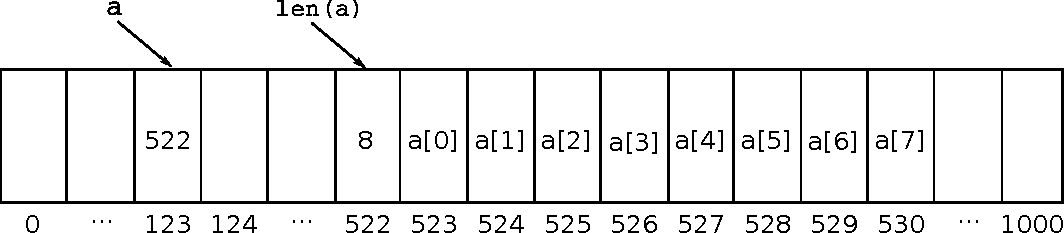
\includegraphics[scale=0.4]{figures/list_rep.pdf}

\smallskip

\tiny Memory representation of list \lstinline{a}
\end{center}
\end{frame}

\begin{frame}[fragile]
Lists are \emph{mutable} objects because we can change their values.

\bigskip

For example, the following code reverses the order of elements in a list \lstinline{a}:

\begin{lstlisting}[language=Python]
n = len(a)
for i in range(n / 2):
    temp = a[i]
    a[i] = a[n - 1 - i]
    a[n - 1 - i] = temp
\end{lstlisting}

\bigskip

One of the most basic operations on a list is to \emph{iterate} over all its elements.

\bigskip

For example, the following code computes the average of a list of floats:

\begin{lstlisting}[language=Python]
total = 0.0
for i in range(len(a)):
    total += a[i]
average = total / len(a)
\end{lstlisting}

and the following code does the same without referring to the indices explicitly:

\begin{lstlisting}[language=Python]
total = 0.0
for v in a:
    total += v
average = total / len(a)
\end{lstlisting}
\end{frame}

\begin{frame}[fragile]
\begin{framed}
\tiny sample.py: Accept integers $m$ and $n$ as command-line arguments. Write to standard output a random sample of $m$ integers in the range $0 \dots n-1$ (no duplicates).
\end{framed}

\begin{lstlisting}[language=Python]
import random
import stdarray
import stdio
import sys

m = int(sys.argv[1])
n = int(sys.argv[2])
perm = stdarray.create1D(n, 0)
for i in range(n):
    perm[i] = i
for i in range(m):
    r = random.randrange(i, n)
    temp = perm[r]
    perm[r] = perm[i]
    perm[i] = temp
for i in range(m):
    stdio.write(str(perm[i]) + ' ')
stdio.writeln()
\end{lstlisting}

\begin{lstlisting}[language={}]
$ python sample.py 6 16
9 6 0 8 5 15 
$ python sample.py 10 1000
389 22 385 925 611 485 866 978 212 298 
$ python sample.py 20 20
7 18 2 16 4 10 14 0 3 13 17 8 5 1 11 6 9 12 19 15 
\end{lstlisting}
\end{frame}

\begin{frame}[fragile]
\begin{framed}
\tiny couponcollector.py: Accept integer $n$ as a command-line argument. Write to standard output the number of coupons you collect before obtaining one of each of $n$ types.
\end{framed}

\begin{lstlisting}[language=Python]
import random
import stdarray
import stdio
import sys

n = int(sys.argv[1])
count = 0
collectedCount = 0
isCollected = stdarray.create1D(n, False)
while collectedCount < n:
    value = random.randrange(0, n)
    count += 1
    if not isCollected[value]:
        collectedCount += 1
        isCollected[value] = True
stdio.writeln(count)
\end{lstlisting}

\begin{lstlisting}[language={}]
$ python couponcollector.py 1000
5821
$ python couponcollector.py 1000
8155
$ python couponcollector.py 1000000
13988284
\end{lstlisting}
\end{frame}

\begin{frame}[fragile]
\begin{framed}
\tiny primesieve.py: Accept integer $n$ as a command-line argument. Write to standard output the number of primes less than or equal to $n$.
\end{framed}

\begin{lstlisting}[language=Python]
import stdarray
import stdio
import sys

n = int(sys.argv[1])
isPrime = stdarray.create1D(n + 1, True)
for i in range(2, n):
    if (isPrime[i]):
        for j in range(2, n / i + 1):
            isPrime[i * j] = False;
count = 0
for i in range(2, n + 1):
    if isPrime[i]:
        count += 1
stdio.writeln(count)
\end{lstlisting}

\begin{lstlisting}[language={}]
$ python primesieve.py 25
9
$ python primesieve.py 100
25
$ python primesieve.py 10000
1229
$ python primesieve.py 1000000
78498
$ python primesieve.py 100000000
5761455
\end{lstlisting}
\end{frame}

\begin{frame}[fragile]
\begin{framed}
\tiny selfavoid.py: Accept integers $n$ and $trials$ as command-line arguments. Do $trials$ random self-avoiding walks in an $n$-by-$n$ lattice. Write to standard output the percentage of dead ends encountered.
\end{framed}

\begin{lstlisting}[language=Python]
import random
import stdarray
import stdio
import sys

n      = int(sys.argv[1])
trials = int(sys.argv[2])
deadEnds = 0
for t in range(trials):
    a = stdarray.create2D(n, n, False)
    x = n / 2
    y = n / 2
    while (x > 0) and (x < n - 1) and (y > 0) and (y < n - 1):
        a[x][y] = True
        if a[x - 1][y] and a[x + 1][y] and a[x][y - 1] and a[x][y + 1]:
            deadEnds += 1
            break
        r = random.randrange(1, 5)
        if   (r == 1) and (not a[x + 1][y]):
            x += 1
        elif (r == 2) and (not a[x - 1][y]):
            x -= 1
        elif (r == 3) and (not a[x][y + 1]):
            y += 1
        elif (r == 4) and (not a[x][y - 1]):
            y -= 1
stdio.writeln(str(100 * deadEnds / trials) + '% dead ends')
\end{lstlisting}
\end{frame}

\begin{frame}[fragile]
\begin{lstlisting}[language={}]
$ python selfavoid.py 5 100
0% dead ends
$ python selfavoid.py 20 100
31% dead ends
$ python selfavoid.py 40 100
77% dead ends
$ python selfavoid.py 80 100
98% dead ends
$ python selfavoid.py 5 1000
0% dead ends
$ python selfavoid.py 20 1000
30% dead ends
$ python selfavoid.py 40 1000
75% dead ends
$ python selfavoid.py 80 1000
98% dead ends
\end{lstlisting}
\end{frame}

\section{Tuples and Sequences}
\begin{frame}[fragile]
blah
\end{frame}

\section{Sets}
\begin{frame}[fragile]
blah
\end{frame}

\section{Dictionaries}
\begin{frame}[fragile]
blah
\end{frame}

\section{Looping Techniques}
\begin{frame}[fragile]
blah
\end{frame}

\end{document}
